\section{External World Interfaces}
\subsection{General Purpose Input-Output Ports (GPIO)}
\subsubsection{General Characteristics of I/O Ports}
\begin{itemize}
	\item Allow comunication with the external world
	\item Operate digitally and can be configured as either inputs or outputs
	\item Can be configured individually or in groups called ports
\end{itemize}
\begin{multicols}{2}
	\subsubsection{Structure of an Input-Output Pin}
	\begin{itemize}
		\item Input Pins, for binary Status
		\item Output Pins, for binary Status
		\item GPIO Interfaces, for General IN or OUT
	\end{itemize}
	
	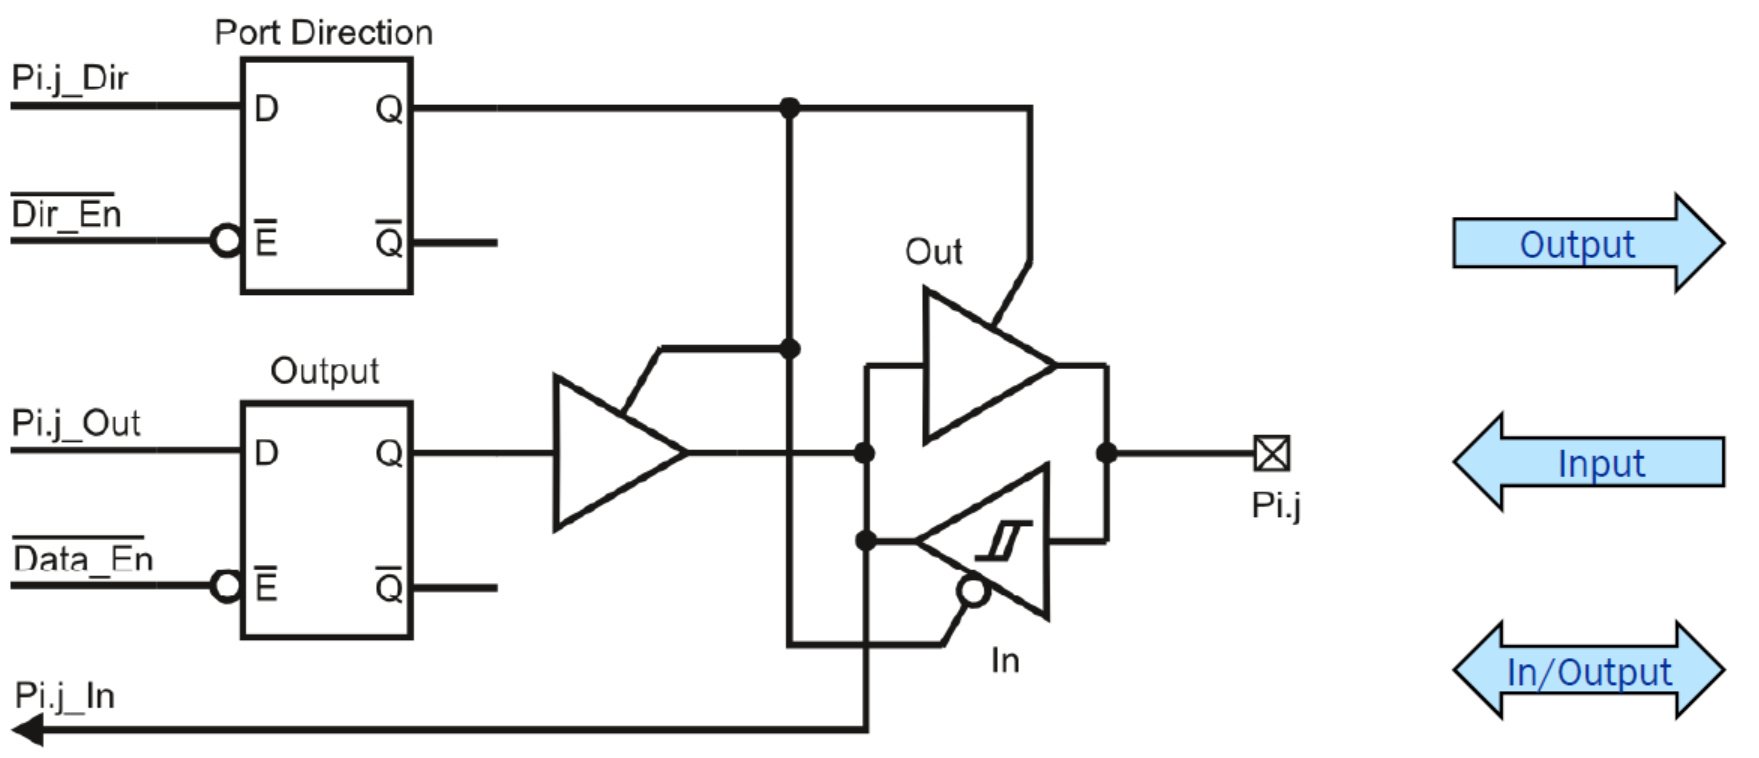
\includegraphics[width=\linewidth]{images/IOStructure}  
\end{multicols}

\subsubsection{MSP430 GPIO Registers}
\begin{tabular}{lll}
	\textbf{PxSEL}   &Port x Function Select             & Sets pin functionality  \\ 
	\textbf{PxDIR}   &Port x Data Direction              & Sets pin as either IN or OUT \\ 
	\textbf{PxOut}   &Port x Out                         & Data-out register \\ 
	\textbf{PxIN}    &Port x Input                       & Data-in register  \\ 
	\textbf{PxIFG}   &Port x Interrupt Flag              & Interrupt request for port x \\ 
	\textbf{PxIES}   &Port x Interrupt Edge Selection    & Sets signal edge to trigge interrupts in Port x input  \\ 
	\textbf{PxIE}    &Port x Interrupt Enable            & Enables interrupts from Port x pins \\ 
	\textbf{PxREN}   &Port x Ressistor Enable            & Enables internal pull-up/down resistors \\ 
	\textbf{PxDS}    &Port x Drive Strength              & Sets driver strength for port pins to up to 30mA  \\ 
	\textbf{PxIV}    &Port x Interrupt Vector            & Priority encoding for port Interrupts \\ 
\end{tabular} 

\subsubsection{Electrical Characteristics in I/O Pins}
\begin{tabular}{lll}
	$ V_{IL} $& Input Low Voltage&Maximum voltage inperpreted as low by pin input buffer\\
	$ V_{IH} $& Input High Voltage& Minimum voltage interpreted as high by pin inpput buffer\\
	$ V_{OL} $& Output Low Voltage& Locig-low level. Minimum voltage oserved at pin outputdriver\\
	$ V_{OH} $& Output High Voltage& Logic-high level. Maximum voltage observed at pin output driver\\
	$ V_M $   & Pin Threshold Voltage& Ultimate level seperating low and high levels in a digital pin\\
	&                      & Specified as $ V_m=V_{DD}/2 $ for CMOS logic\\
\end{tabular} 

\clearpage